\section{模型检验}
\label{sec:validation}
\label{sec:evaluation}

本节按``数值可信度''与``物理结构性局限''两类分别陈述检验结果。前者回答``在给定的方程与边界下，数值解算得准不准''；后者回答``给定的方程与边界是否足以描述真实烘干过程''。两类问题不能互相替代，这一点是本节的行文原则。

\subsection{离散守恒审计}

在有限体积离散下，所有内部界面通量在总体收支中成对抵消，故含水率的总量变化必须精确等于表面传质通量的累积值。定义归一化含水率总量 $\sum_iV_i{\C}_i$ 与累积失水量，本文在每一个输出时刻检验

\begin{equation}
\sum_iV_i{\C}_i(\t)+\int_0^\t\frac{\hmass}{\R}\left[\C(\R,s)-\Cinf(s)\right]\mathrm{d}s
=\sum_iV_i{\C}_i(0),
\label{eq:massaudit}
\end{equation}
其实测相对残差为：问题一 \QOneMassError，问题二 \QTwoMassError，问题三 \QThreeMassError，问题四 \QFourMassError（网格加密各档的结果见表~\ref{tab:validation-grid}）。这些残差都在机器精度量级，说明\textbf{离散格式的质量收支是闭合的}。对问题四而言，这一检验尤其有意义：式\eqref{eq:massaudit} 是在材料测度下成立的，若式\eqref{eq:cancel} 的相消被误加或多加了对流项，或者式\eqref{eq:rhod} 的幂次写错，残差会立刻变成 $O(1)$。

能量方面的结论要谨慎一些。问题一的物性为常数，可以把 $\rho\cp$ 提出积分号，从而检验``域内显热变化 $=$ 累积对流换热''这一积分恒等式，实测相对残差为 \QOneEnergyError。问题二$\sim$四则\textbf{不能}做同样的检验：式\eqref{eq:q2system} 中的 $\rho\cp$ 随含水率变化，无法从时间导数中提出，因此$\int\rho\cp(\T-{\T}_0)\mathrm{d}V$ 并不是该方程所守恒的量。本文对这三问只检验\textbf{瞬时}收支恒等式，即每一时刻都满足

\begin{equation}
{\R}^2\sum_iV_i\,\rho_i{\cp}_i\frac{\mathrm{d}{\T}_i}{\mathrm{d}\t}=F^T_{\Nr-1/2}=\R\hconv(\Tinf-{\T}_s),
\end{equation}
并明确\textbf{不声称} $\rho\cp\T$ 的积分守恒。把问题一的积分守恒结论搬到后三问，是一个很容易犯而后果不小的错误，故在此显式区分。

\subsection{空间网格加密}
\label{sec:conv}

以 $\Nr=641,1281,2561,5121$ 四档网格求解同一问题，把结果插值到题目指定的输出网格上比较相邻两档的最大差值，结果见表~\ref{tab:validation-grid}（网格收敛与 Richardson 估计的做法见文献~\cite{roache1998}）。

\geninput{tab/validation_grid}{网格加密验证表由 \texttt{make tables} 从 \texttt{results/validation/accuracy*.json} 生成。}

由表~\ref{tab:validation-grid} 可见，相邻网格的场量差按约四倍缩小，与二阶空间离散的预期一致：问题一的最大温度差依次为 $4.82\times10^{-6}$、$1.37\times10^{-6}$、$2.89\times10^{-7}$~K（比值约 $3.5$、$4.7$），$2561$ 与 $5121$ 两档之差已小于 $3\times10^{-7}$~K 与 $2.3\times10^{-7}$~kg/kg，\textbf{远小于交付要求的四位小数分辨率}（$10^{-4}$），故正式计算取 $\Nr=2561$ 是充分的。

\textbf{其二，终点时刻对网格的依赖更弱，且收敛更快。} 问题三的终点时刻差由 $0.2137$~s 降到 $0.0534$~s 与 $0.0134$~s（相邻档比值约 $4.0$、$4.0$），问题四由 $7.0\times10^{-3}$~s 降到 $1.7\times10^{-3}$~s 与 $6.2\times10^{-4}$~s。也就是说，$\Nr$ 加倍带来的终点时刻变化在正式网格上只有 \QThreeGridEventDiff~s（问题三）与 \QFourGridEventDiff~s（问题四），\textbf{比报出的小时位数（$10^{-4}$~h $=0.36$~s）小两到三个数量级}。这从数值上支持了``烘干时长可以作为答案报出''这一主张。

\textbf{其三，终点判据本身依赖网格，但依赖很弱。} 表~\ref{tab:validation-grid} 的``终点时刻差''列同时反映了两件事：解本身的收敛，以及``全场最大值''这一泛函对网格的敏感性（网格越细，最大值越大，达标越晚）。两者在本例中都只有秒量级，故判据的网格依赖性不构成对结论的威胁。若把判据改为断面平均值，终点时刻会明显缩短，但那是另一个问题（假设 B3 已把这一选择及其代价写明）。

\subsection{时间积分精度}
\label{sec:timecheck}

为把时间误差与空间误差分离，本文做了两组检验，结果见表~\ref{tab:validation-time}。第一组在\textbf{同一空间网格}上把时间积分方法由变阶 BDF 换成五阶 Radau IIA，两者解的差异即时间方法的离散误差；第二组把相对/绝对容差各收紧十倍、最大步长减半，考察误差控制的可靠性。两种时间方法分别对应文献~\cite{ascher1998}与 SciPy 的 Radau IIA 实现~\cite{scipyradau2026}，本文使用的事件检测机制见~\cite{scipyivp2026}。

\geninput{tab/validation_time}{时间精度交叉验证表由 \texttt{make tables} 从验证报告目录 \texttt{results/validation/} 中的 JSON 文件生成。}

由表~\ref{tab:validation-time}：在 $161$ 节点网格上，两种时间方法的温度差在 $1.3\times10^{-8}\sim1.6\times10^{-8}$~K、含水率差在 $3.9\times10^{-10}\sim4.5\times10^{-10}$~kg/kg 量级，\textbf{比同一网格上的空间离散误差小两到三个数量级}，说明时间误差不是当前精度的限制因素。终点时刻的差异同样很小：问题三为 $2.06\times10^{-6}$~s、问题四为 $5.55\times10^{-4}$~s，即事件定位的可靠性远高于报出的位数要求。第二组检验（容差收紧、步长减半）给出的差异同样是场量 $10^{-6}$~K、$10^{-9}$~kg/kg、终点 $5.2\times10^{-5}$~s 量级，与第一组一致。

\begin{figure}[!ht]
  \centering
  \IfFileExists{figs/fig-validation.pdf}{%
    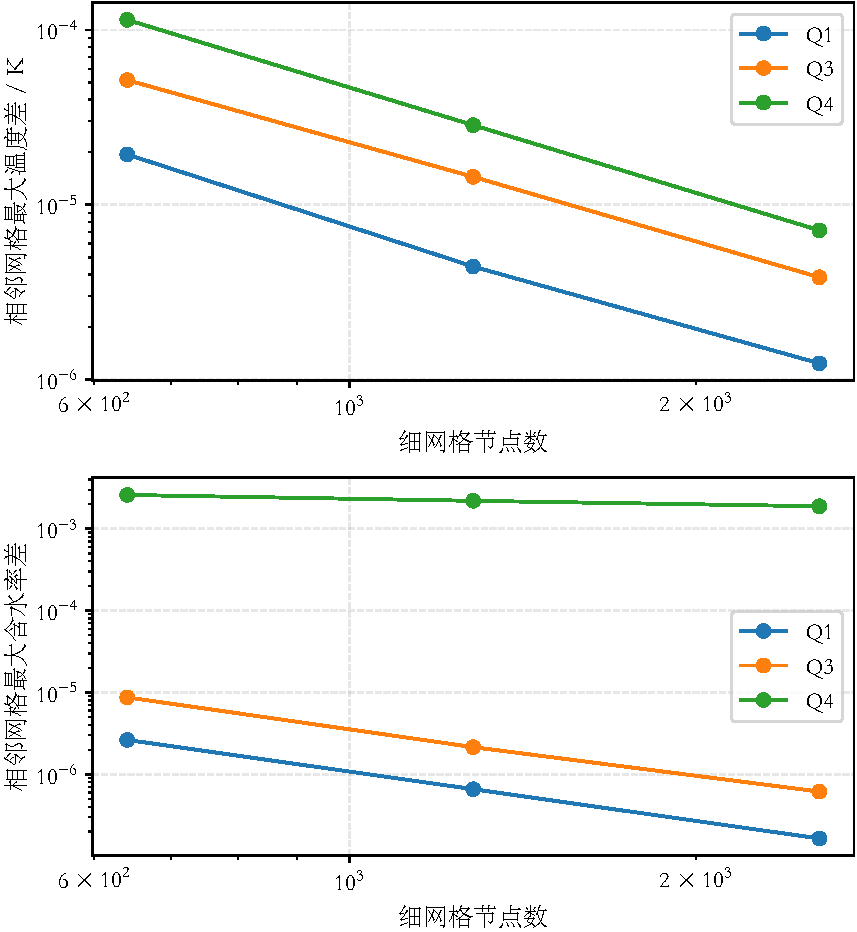
\includegraphics[width=0.68\linewidth]{figs/fig-validation.pdf}%
  }{%
    \instruction{【插图缺失】未找到 \texttt{figs/fig-validation.pdf}，请先运行 \texttt{make figs}。}%
  }
  \caption{数值验证汇总。(a) 四问的相邻网格最大温差随节点数下降，虚线为二阶参考斜率；(b) 同一网格上 BDF 与 Radau IIA 的差异；(c) 环境外推假设的灵敏度}
  \label{fig:validation}
\end{figure}

图~\ref{fig:validation}(a) 把表~\ref{tab:validation-grid} 的温度列画在双对数坐标上，四问的数据点基本平行于二阶参考线，说明\textbf{空间离散在四问中都表现出二阶收敛}；图~\ref{fig:validation}(b) 直观显示时间方法的差异比空间差异小两个数量级。

\subsection{与圆柱 Bessel 级数解析解的对照}
\label{sec:analytic}

数值解与自身的加密解比较只能说明``收敛''，不能排除``收敛到错误的方程''。为此本文为问题一的温度方程构造了独立参考解：取与环境一致的恒定环境温度与恒定的初始温度，圆柱内一维导热问题在 Robin 边界下可用 Bessel 函数级数表示

\begin{equation}
\frac{\T(\rpos,\t)-\Tinf}{{\T}_0-\Tinf}
=\sum_{n=1}^{\infty}A_n\,J_0\!\left(\mu_n\frac{\rpos}{\Rzero}\right)\exp\!\left(-\frac{\mu_n^2\alpha \t}{{\Rzero}^2}\right),
\qquad
A_n=\frac{2\,\mathrm{Bi}}{J_0(\mu_n)\left(\mu_n^2+\mathrm{Bi}^2\right)},
\label{eq:bessel}
\end{equation}
其中 $\mu_n$ 是特征方程 $\mu J_1(\mu)=\mathrm{Bi}\,J_0(\mu)$ 的正根，$\mathrm{Bi}=\hconv\Rzero/\kcond$，$\alpha=\kcond/(\rho\cp)$。由于附件 1 的环境温度是分段线性的，本文对实测驱动逐段做卷积叠加（即把分段线性驱动视为阶跃序列的叠加），从而得到一个\textbf{与数值解共享同一驱动、但计算方法完全独立}的参考解。

实测结果：模态数由 $512$ 增到 $1024$ 时参考解自身的最大变化为 \QOneBesselModes~K（即参考解已收敛到 $10^{-9}$~K 量级）；与数值解相比，最大温度误差为 \QOneBesselNTwoFiveSixOne~K（$\Nr=2561$）与 \QOneBesselNFiveOneTwoOne~K（$\Nr=5121$），$641$ 节点时为 $5.36\times10^{-6}$~K。误差随网格加密按约 $14.7$ 倍的比值下降（网格加倍约对应四倍，此处因同时收紧时间容差而更快），\textbf{这既验证了数值解正确求解了温度方程，也再次确认了空间离散的二阶性质}。这是本文最强的一项独立验证。

\subsection{物理合理性检查}

除数值精度外，本文还对解做了若干物理一致性检查，全部通过：

\begin{itemize}
  \item \textbf{含水率单调不增}：所有节点上 $\C$ 随时间是单调不增的，最大正向跳变在 $10^{-15}$ 量级（浮点舍入），未出现虚假回升；
  \item \textbf{径向单调性}：每一时刻都有 $\C$ 由轴心向表面单调递减，即干燥由表及里，与边界条件的符号方向一致；
  \item \textbf{温度不超调}：所有时刻与位置都满足 $\T\le\max_t\Tinf(\t)$，未出现高于环境温度的过冲；
  \item \textbf{环境波动引起的小幅温度回落是数据驱动而非数值不稳定}：附件 1 的实测温度序列并非单调上升（含有 $95$ 个下降步，最大单步降幅 $0.45$~K），故药材温度在 $2\sim4$~h 出现约 $10^{-3}$~K 的轻微回落；
  \item \textbf{退化检验}：问题四中把半径置为常数后，材料坐标方程与固定半径方程\textbf{逐位相同}（差值严格为 $0$），验证了式\eqref{eq:cancel} 的相消与实现的一致性；
  \item \textbf{域外留空的严格性}：问题四的交付文件中，落在当时药材之外的列必须留空、域内与表面列必须为有限值；程序对两者都做硬校验，任一条不满足即报错。
\end{itemize}

\subsection{格式与可复现性}

交付文件 \texttt{result1$\sim$4.xlsx} 的工作表名、列数、表头、时间步长与小数位数均由程序按题目模板硬校验后才写出，四个文件的实测结构为：\texttt{result1}、\texttt{result2} 各含``温度''与``水分浓度''两张工作表、$1$~s 步长；\texttt{result3}、\texttt{result4} 各含一张工作表、$60$~s 步长，\texttt{result4} 的末列是文字``药材表面''。所有数值保留四位小数。

为验证结果可复现，本文在独立目录中重新执行了完整的四问计算，并把新结果与交付文件逐单元格比较：时间列、距离列、温度场与含水率场的最大差异全部为 $0$，工作表的 XML 内容完全一致。同时，每个问题的清单文件记录了输入文件（题面、附件 1、附件 2、模板）与全部源程序的 SHA-256 摘要，以及求解所记录的运行参数，使``论文中的数字来自哪一次运行、用哪一版代码''可以追溯。

\subsection{环境外推的灵敏度分析}
\label{sec:sensitivity}

假设 B2 把 $4$~h 之后的环境条件固定为附件 1 的末值（$\Tinf=50.165~^\circ$C、$\Cinf=0.04986$~kg/kg），而这一外推覆盖了问题 2/3/4 全程约 $93\%$ 的时长。为量化其影响，本文以附件 1 末小时内 $\Tinf$、$\Cinf$ 的\textbf{实测最小值与最大值}相对末值的偏移作为扰动幅度（该偏移量本身由数据决定：附件 1 末小时内 $\Tinf$ 相对末值 $50.165~^\circ$C 的偏移为 $-0.408$~K 与 $+0.071$~K，$\Cinf$ 相对 $0.04986$~kg/kg 的偏移为 $-1.1\times10^{-4}$ 与 $+3.8\times10^{-4}$~kg/kg），重新求解并比较终点时刻。

\geninput{tab/sensitivity}{灵敏度表由 \texttt{make tables} 从 \texttt{results/validation/numerics.json} 生成。}

由表~\ref{tab:sensitivity} 可以得到三条结论。

\textbf{其一，结果对末值温度的敏感度远大于对末值含水率的敏感度。} 把末段温度整体下移 $0.408$~K 使问题三的烘干时长增加 $0.746$~h（$+1.30\%$）、问题四增加 $0.654$~h（$+1.29\%$）；而把末段含水率上下扰动 $10^{-4}$~kg/kg 量级只使终点变化 $0.002\sim0.009$~h（不足 $0.02\%$）。两者相差约两个数量级。原因是烘干时长由内部扩散控制，而扩散系数对温度是指数敏感（式\eqref{eq:app3} 的 $e^{-3850/\T}$），对边界浓度差只是线性敏感。

\textbf{其二，外推假设带来的不确定性是``小时量级''，小于模型的结构性不确定性。} 温度扰动引起的 $0.65\sim0.75$~h 是该假设下的最大偏差；而第~\ref{sec:limitations} 节列出的物理闭合问题（尤其是未计入蒸发潜热）无法用本题数据量化，且方向上是``使干燥偏快''。因此在报告结论时，应把``约 $57$~h''理解为在当前假设下的模型预测值，而不是具有小时级置信区间的实验预测。

\textbf{其三，该灵敏度分析支持``继续按末值保持外推''这一选择。} 若把末段环境温度按``最优情形''（取末小时最大值）处理，烘干时长为 $57.04$~h；按``最差情形''（取末小时最小值）为 $57.91$~h。两者与该小时的时间分辨率（题面以小时为单位报告）相比仍在同一数量级内，说明结论的定性判断（约 $2\sim2.4$ 天）不因这一外推而改变。

\subsection{模型的结构性局限}
\label{sec:limitations}

上述验证只覆盖``数值是否算准''，下列局限则属于\textbf{模型本身}，不能靠加密网格或收紧容差消除，必须如实列出：

\begin{enumerate}
  \item \textbf{表面热边界不含蒸发潜热（假设 A5）}。题目未给出水的汽化潜热与蒸发速率的关系式，本文没有凭空补一个参数，代价是表面温度可能偏高、干燥速率可能偏快。这一缺失在 $2\sim3$ 天的长时间干燥中影响明显大于 $30$~min 的预热阶段，且\textbf{其大小无法用本题数据量化}。若要评估，需要补充表面温度或蒸发速率的实测数据。
  \item \textbf{传质边界是有效闭合而非已验证的物理关系（假设 A7）}。题目给出的 $\hmass$ 与 $\Cinf$ 组合成了浓度差驱动的边界条件，但题目未说明气相水分的 kg/kg 与药材干基含水率的 kg/kg 是否同一基准（两者数值相差约 $51$ 倍）。若基准不一致，边界驱动势会整数量级地偏，烘干时长随之整体偏移。这是本文结论中不确定性最大的一环。
  \item \textbf{$4$~h 之后的环境条件是外推（假设 B2）}。该外推覆盖全程 $93\%$ 的时长，影响量级已在第~\ref{sec:sensitivity} 节量化为小时量级。
  \item \textbf{几何与收缩的简化（假设 A1、A10）}。端面效应被均摊进径向模型，无法用题目数据约束；长度不变的假设使``整块药材体积变化''这一报送口径存在两种可能（体积剩 $21.5\%$ 或 $35.9\%$），附件 2 的数据无法区分。
  \item \textbf{问题四的收缩效应结论依赖于传质闭合}。第~\ref{sec:q4result} 节得到的``收缩使干燥加快''是在``干基通量形式''的闭合下成立的；若改用按表面积的蒸气通量闭合，``面积减小''的减速效应会重新出现。本文不通过添加对流项的方式人为制造这一效应（那是重复计入，见第~\ref{sec:cancellation} 节），但也不声称该结论对闭合形式不敏感。
  \item \textbf{不引入平衡含水率（假设 A11）}。题目只给终点判据、未给吸附等温线，故本文不声称存在使干燥停滞的正平衡含水率；末期表面含水率渐近趋近但不低于 $\Cinf$，这是模型的直接后果而非物理结论。
  \item \textbf{四位小数是输出格式而非物理精度（假设 B4）}。交付文件按题目要求保留四位小数，但模型的物理预测精度受上述结构性假设限制，两者不可混淆。
\end{enumerate}

需要说明的是，第 1、2、5 条都属于\textbf{闭合关系的形式}层面：它们不改变方程的结构，也不影响数值验证的结论，但会整体平移预测值。若将来获得表面温度、气相湿度定义或吸附平衡数据，应\textbf{先修订物理闭合、再重新验证}，而不是通过加密网格来``改善''这些误差。
